\documentclass[final,leqno]{siamltex}

\usepackage{amsmath,amssymb,amsfonts,algorithm,algorithmic,multirow,booktabs,graphicx}
\DeclareMathOperator{\prox}{prox}

\title{OUR REPORT TITLE\thanks{This report was conducted as part of the Columbia ECBM E6040 final project.}} 

\author{Zichen Chao\footnotemark[2] \and Shenlong Gu\footnotemark[2] \and Kan Zhu\footnotemark[2] \and Yibo Zhu\footnotemark[3]}

\begin{document}
\maketitle

\renewcommand{\thefootnote}{\fnsymbol{footnote}}

\footnotetext[2]{Department of Computer Science, Columbia University in the City of New York.}
\footnotetext[3]{Department of Industrial Engineering and Operations Research, Columbia University in the City of New York.}

\slugger{siopt}{xxxx}{xx}{x}{x--x}
\begin{abstract} 
In this paper, we realize the result of the paper ReNet: A Recurrent Neural Network Based Alternative to Convolutional Networks \cite{renet} using Python's Deeplearning Library $\textit{Theano}$.

\end{abstract} 

\begin{keywords}
Recurrent Neural Networks, Convolutional Neural Networks, Theano
\end{keywords}

\pagestyle{myheadings}
\thispagestyle{plain}

\section{Introduction}
\subsection{Motivation}
Convolution Neural Networks(CNN) have proven its power in object recognition and image classification problems. Previous works of Recurrent Neural Networks(RNN) also shows great performance in handwriting recognition/generation and speech recognition. Rather than the multi-dimensional RNN inspired before, one could use a uni-dimensional RNN, which makes each output activation of the layer be computed with respect to the whole input image, rather than the local extracted activation computed in CNN. Also, comparing to multi-dimensional RNN, the number of RNNs at each layer scales could be linear with respect to the number of dimensions $d$ of the input image ($2d$), while multi-dimensional RNN requires the exponential number of RNNs at each layer ($2^d$). Furthermore, parallelizability could be easier, as each RNN is dependent only along a horizontal or vertical sequence of patches. 
\subsection{Related Work}
The idea of using RNN on offline handwriting recognition is from Graves and Schmidhuber's paper\cite{multidimrnn}. They use Multi-dimensional RNN (MDRNN), which avoids any alphabet specific preprocessing and thus could be applicable for any language, with the help of connectionist temporal classification algorithm. The challenging part of offline problem comparing to online problem is that the input is no longer one dimensional, hence if the image shifts vertically by one pixel, it would be completely different. 
Other related works aiming at classification of images is summarized in a github website \cite{imgcls}. 

\subsection{Organization}

The rest of the paper is organized as follows. We review the model architecture of ReNet in \S \ref{background}. Then we propose our implementation of ReNet in \S \ref{implementation}. In \S \ref{result} we recreate the result of ReNet. Lastly, \S \ref{discussion} concludes the paper and gives direction for future work.

\section{Background} \label{background} 
The ReNet paper proposed a deep neural network architecture for object recognition based on recurrent neural networks(RNN). The proposed network, called ReNet, replaces the ubiquitous convolution+pooling layer of the deep convolutional neural network with four recurrent neural networks that sweep horizontally and vertically in both directions across the image. \\

First, we sweep the image vertically with two RNNs, with one RNN working in a bottom-up direction and the other working in a topdown direction. Each RNN takes as an input one (flattened) patch at a time and updates its hidden state, working along each column $j$ of the split input image $X$.\\

After this vertical, bidirectional sweep, we concatenate the intermediate hidden states (forward and backward) at each location of patch to get a composite feature map. Each state is now the activation of a feature detector at the corresponding location with respect to all the patches in the $j$-th column of the original input. Next we sweep over the obtained feature map horizontally with two RNN. In a similar manner as the vertical sweep, these RNNs work along each row resulting in the output feature map. Now, each vector represents the features of the original image patch in the context of the whole image.\\

The functions are as follows:
\begin{eqnarray}
	v_{i,j}^F = f_{VFWD}(z_{i,j-1}^F, p_{i,j}) \text{~for } j=1,\dots,J \nonumber \\
	v_{i,j}^R = f_{VREV}(z_{i,j+1}^R, p_{i,j}) \text{~for } j=J,\dots,1 \nonumber
\end{eqnarray}

The schema is as follows:\\
\begin{center}
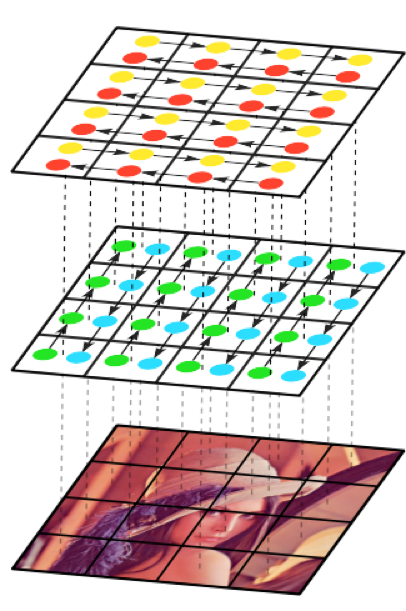
\includegraphics[scale=0.45]{Figures/onelayer_renet}
\end{center}

They evaluate the proposed ReNet on three widely-used benchmark datasets; MNIST, CIFAR-10 and SVHN. The result suggests that ReNet is a viable alternative to the deep convolutional neural network, and that further investigation is needed.

\section{Implementation} \label{implementation}
\subsection{Data Preprocessing}
It is well-known that augmenting training data often leads to better generalization. We employed a shifting augmenting strategy. In the case of shifting, we either shifted the image by $2$ pixels to the left ($25\%$ chance), $2$ pixels to the right ($25\%$ chance) or left it as it was. After this first processing, we further either shifted it by $2$ pixels to the top ($25\%$ chance), $2$ pixels to the bottom ($25\%$ chance) or left it as it was. This two-step procedure makes the model more robust to slight shifting of an object in the image. The shifting was done without padding the borders of the image, preserving the original size but dropping the pixels which are shifted out of the input while shifting in zeros. The choice of whether to apply these augmentation procedures on each dataset was chosen on a per-case basis in order to maximize validation performance.\\

Here is snapshots on parts of our data augmentation code:\\

\begin{center}
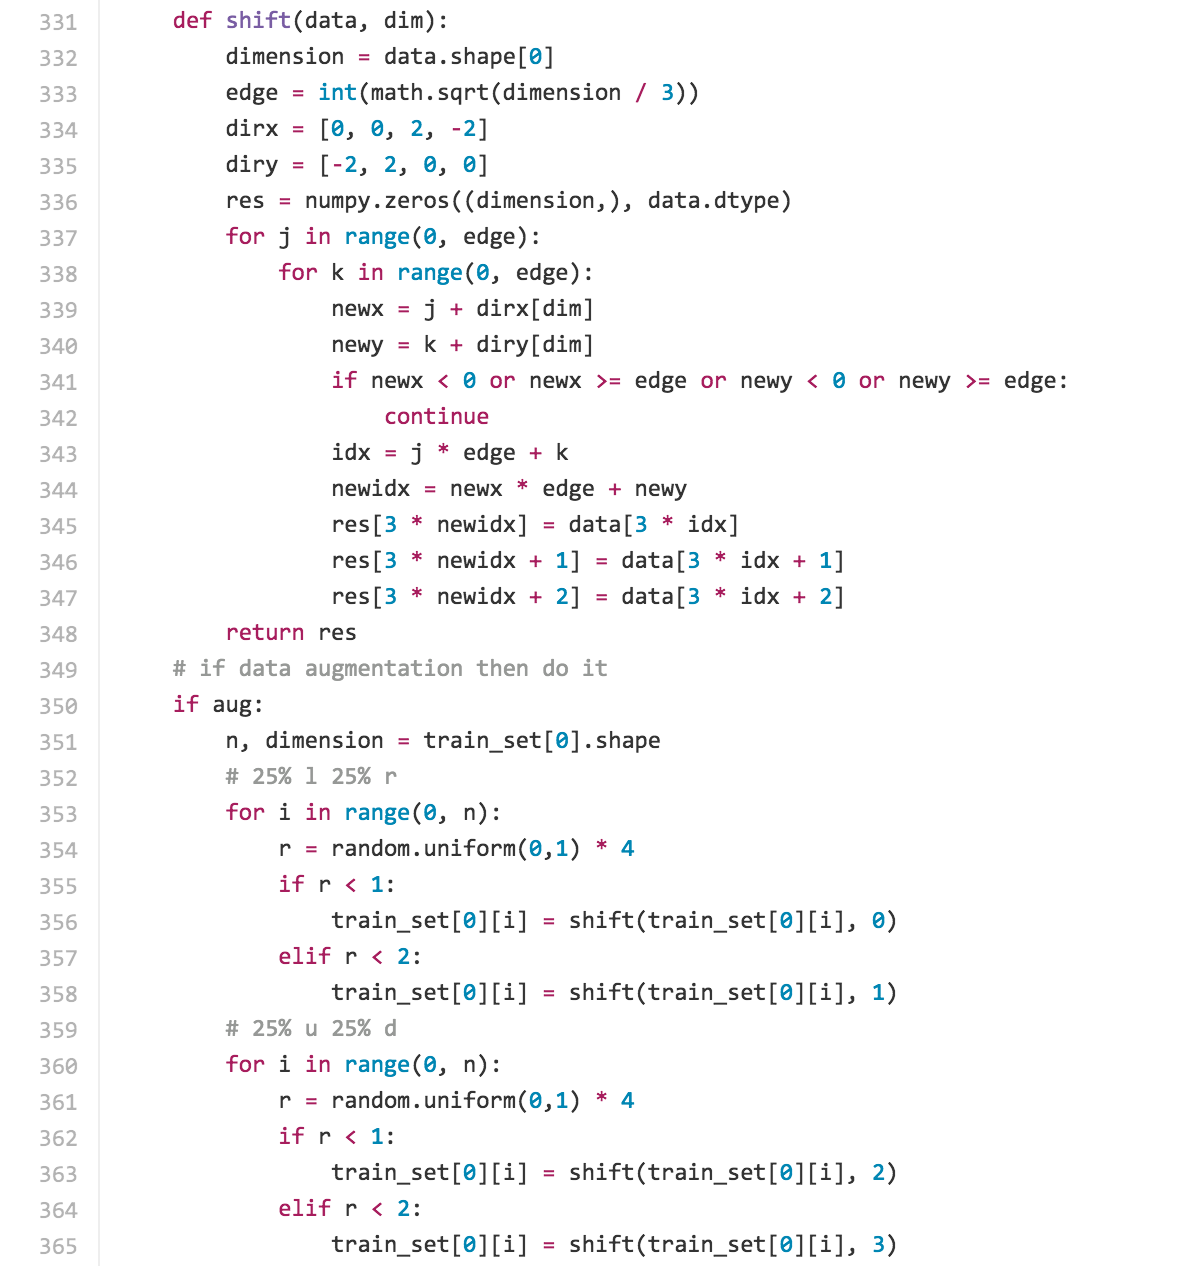
\includegraphics[scale=0.6]{Figures/data_aug}	
\end{center}

Meanwhile, we also pre-processed image data by scaling its original pixel to be mean zero.

\subsection{Adaptive Learning Rate}
We applied adaptive learning rate algorithm to achieve better test accuracy. Based on what have learned in class, we proposed a very straightforward algorithm to set the adaptive learning rate. The basic idea is if we find the discrepancy between validation errors of two consecutive steps are very small, we think the learning rate maybe too large which cannot approximate optimal value well. So we reduce the learning rate at this time. And we should speed up the learning rate reduction as training process goes further. Because the more we are closed to the optimal point, the smaller step we need to choose and the more cautious we should be at learning rate. Therefore, we’ve tried several methods of learning rate reduction. Experiments told us our choice works well. The following code shows how we changed the learning rate:\\

\begin{center}
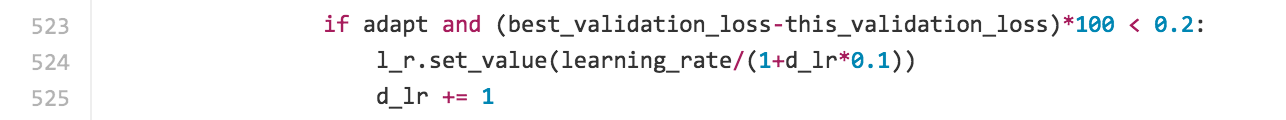
\includegraphics[scale=0.55]{Figures/learning_rate}
\end{center}

\subsection{Neural Network Implementation}
For a ReNet layer, first, we sweep the image vertically with two RNNs, with one RNN working in a bottom-up direction and the other working in a topdown direction. Each RNN takes as an input one (flattened) patch at a time and updates its hidden state, working along each column j of the split input image. After this vertical, bidirectional sweep, we concatenate the intermediate hidden states (forward and backward) at each location of patch to get a composite feature map. Each state is now the activation of a feature detector at the corresponding location with respect to all the patches in the j-th column of the original input. Next we sweep over the obtained feature map horizontally with two RNN. In a similar manner as the vertical sweep, these RNNs work along each row resulting in the output feature map. Now, each vector represents the features of the original image patch in the context of the whole image. Moreover, the hidden state of each RNN that we used is Gated recurrent units. The hidden state of the GRU at time t is computed by \cite{DBLP:journals/corr/ChoMGBSB14}:
\begin{eqnarray*}
	h_t &=& (1-\mu_t)\odot h_{t-1}+\mu_t\odot \bar h_t\\
	\bar h_t &=& \text{tanh} (Wx_t+U(r_t \odot h_{t-1})+b)\\
	\lbrack u_t;r_t \rbrack &=& \sigma(W_g x_t+U_g h_{t-1}+b_g)
\end{eqnarray*}
For the actual code design, we find the similarity of this paper and the traditional convolutional neuron network, and just replace the homework 3 convolution layer with our renet layer (with a following mlp), and write the function test\_renet with some adjustable parameters to get experiment results.
\section{Result} \label{result}
We've tested the model under multiple combination of hyper-parameters for the CIFAR-10 dataset, and here is what we get:
\begin{center}
\text{CIFAR-10}
\end{center}
\begin{center}
\begin{tabular}{l c c c c c c r}
\hline
\#Schema & $d$ & $hu$ & $h$ & $batch$ & $aug$ & $adapt$ & Test error\\
\hline
with augmentation & 80 & 500 & 1 & 200 & T & T & 29.41\%\\
without augmentation & 80 & 500 & 1 & 200 & F & T & 28.21\%\\
less hidden state of renet & 40 & 500 & 1 & 200 & F & T & 28.67\%\\
less hidden unit of mlp & 80 & 200 & 1 & 200 & F & T & 29.76\%\\
more hidden layer of mlp & 80 & 200 & 4 & 200 & F & T & 31.42\%\\
No adapt learning & 80 & 500 & 1 & 200 & F & F & 29.97\%\\
Best & 256 & 512 &  1 & 50 & F & T & 21.90\%\\
\hline
\end{tabular}	
\end{center} 
~\\
We set $d$ as the number of hidden units in each ReNet layer, $hd$ as the number of hidden units in each layer, $h$ as the number of hidden layer, $batch$ as the batch size, $aug$ as whether we use data augmentation preprocessing, $adapt$ as whether we use adaptive learning rate.\\

We've also tested the model for MNIST dataset, we managed to get $1.53\%$ test error given the parameter set as $\{d, hu, h, batch, aug, adapt\}=\{40, 250, 1, 200, F, F\}$.\\

The test results are summarized in the above table. The first two columns show that with data augmentation, we do not gain a test error decrease, instead, the test error increased slightly. The $2$nd and the $3$rd column shows that we reduce the test error by $0.4\%$ with higher number of units in ReNet layer. The 2nd and the 4th column show that we reduce the test error by $1\%$ with higher number of hidden units. The 4th and 5th column shows that we reduce the test error by $2\%$ with less number of hidden units in MLP. The 2nd column and 6th column show that we reduce the test error by $2\%$ with adapted learning rate.\\

This is part of our main function implementing the ReNet model:\\
\begin{center}
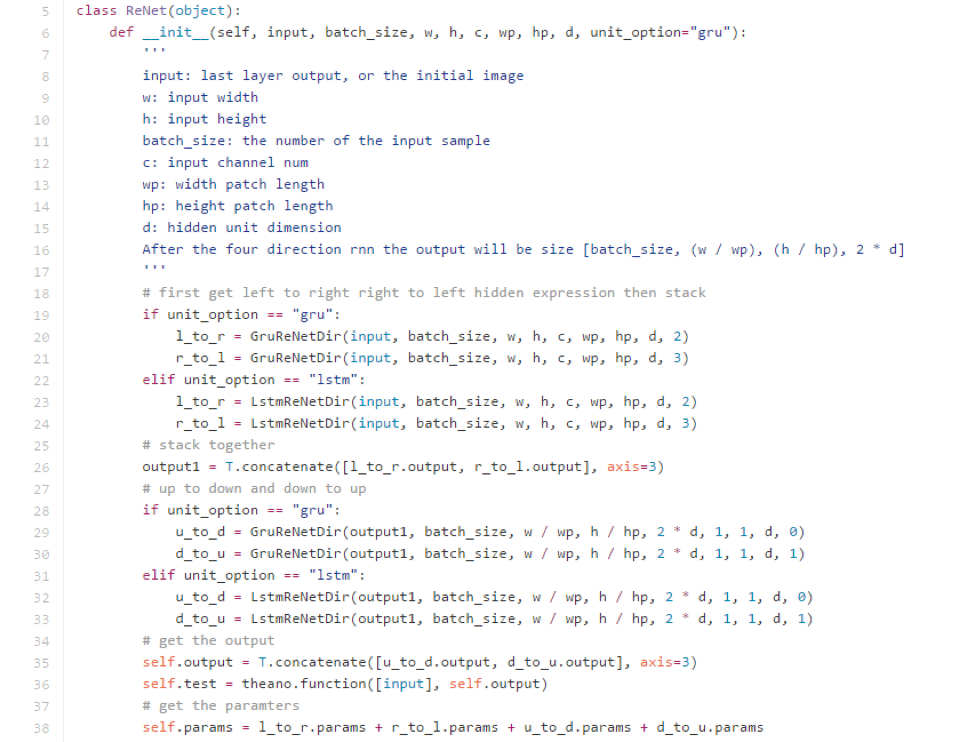
\includegraphics[scale=0.8]{Figures/algo}	
\end{center}

\section{Discussion} \label{discussion}
We successfully implemented the ReNet model. The result is perfect comparing to some previous works. However, we need to be fully aware of some problems we are facing:\\

First, computing power limits. We've tested our model on AWS GPU instance with $1 \times$ NVIDIA GRID GPU (Kepler GK104) and $8 \times$ hardware hyperthreads from an Intel Xeon E5-2670. This is the best configuration that we could afford and access now. However, this also limits the training performance. Hence the hyper-parameters aren't fully tested. One could observe that our best performance happens when we choose larger parameters for hidden units and dimension of ReNet layers.\\

Second, time limit. Due to the fact that this project is due within two weeks, we don't have sufficient time to fully test the performance of the ReNet model.\\

Thirdly, budge limit. We have spent more than 300 dollars on this projects. Although we fully devote ourselves into this project, these are really serious obstacles spotted on our way to pursue perfectness. \\

\subsection{Future Work}
First, we evaluated the proposed ReNet only quantitatively. However, the accuracies on the test sets do not reveal what kind of image structures the ReNet has captured in order to perform object recognition. Further investigation along the line of regularization of neural networks using dropconnect is necessary, as well as exploring ensembles which combine RNNs and CNNs for bagged prediction.\cite{DBLP:journals/corr/BellZBG15} \cite{DBLP:journals/corr/ChenBPMY15}\cite{DBLP:journals/corr/HeH0LT15}\cite{DBLP:journals/corr/KalchbrennerDG15}\cite{DBLP:journals/corr/ZuoSWLWW15} \\

Second, we can use many parallelization tricks which are widely used for training CNN such as parallelizing fully-connected layers, having separate sets of kernels/features in different processors and exploiting data parallelism.\\

Third, this mechanism can be applied to multidimensional grid other than image. We can applied the algorithm to 3D real object detection.
\section*{Contribution}
Zichen Chao analyzed the algorithm, did the coding part, debugged the program, optimized the model performance. Shenlong Gu designed the whole system of ReNet, analyzed the algorithm, optimized the performance, and did the coding part. Kan Zhu analyzed the algorithm, optimized the performance, wrote the report and refined the model. Yibo Zhu analyzed the model, raised algorithmic suggestions, debugged the codes and wrote the report.\\
\bibliographystyle{siam.bst}
\bibliography{bibl}

\end{document}